\chapter{Languages}
\label{chp:languages}
This chapter will explain which programming languages are used in this project. Why they are used and in some cases compare them to other solutions.\\
\subsection*{Front-end}
\label{sec:frontend} % INSERT CORRECT LINKS
HTML, CSS and JS will be used to develop the interface both for desktop and mobile devices. This selection is due to the fact that websites have no real alternatives. This project will not focus on developing for older web browsers hence it will be written in entirely HTML5 without regards to it not working in older browsers such as IE6.

\subsection*{Web-server}
\label{sec:webserver} % INSERT CORRECT LINKS
On the web-server there is the option to use a lot of different languages for implementing the back-end. To name a few: Java Servlets, ASP.NET, PHP, Ruby and Python. As the intention is that the software produced in this project is built on Open Source technologies and software. ASP.NET will not be considered any further even though mod\_ mono and other open source implementations exist simply as these do not offer the complete set of API available. When talking PHP vs Ruby and Python it generally is a tie in . But the ease with which one can set-up a test development on ones localhost is is big plus for PHP. Performance wise it depends heavenly on which type of application is run. Benchmarks shows in different favours. PHP and Java Servlets both have god and bad reputation depending on what area is looked into. The same is true for performance where there are reports showing in the favour of both. Some will argue that general code security is better in Servlets than in PHP while others will argue that it is completely the opposite that is the truth. \\
As the field is under constant development. One version of one of the systems might be far better performance wise but it still depends on what it is used for. The selection comes from what the group has of prior knowledge and experience and hence the selection is PHP as this is where the group feels most comfortable.


\subsection*{Arduino}
\label{sec:arduino} % INSERT CORRECT LINKS
The main programming languages used when programming for Arduino is C \& C++. This is therefore selected for the project and it enables the direct use of shields that are needed for the network and NFC communication. 

\subsection*{Back-end}
\label{sec:backend} 
The back-end of the system that communicates directly with the Arduino and in long term other devices can be designed in a number of different languages. This including PHP. The choice is therefore straight forward as the complete server side system then can run completely in PHP and no extra software is needed.

\subsection*{Language Support}
\label{sec:langSupport}
Localization is something that when designing a system is easy to take into account. But when the system is developed and near completion it can be difficult to implement. Therefore this will be taken into account from the start and in such a way that it supports most common languages.

\subsection*{Folder Structure}
\label{sec:folderStructure}
When designing a system which is supposed to come with a high maintainability it is important to design a usable folder structure. The folder structure of this project can be seen in figure \ref{fig:folderStructure}.\\
\\

\begin{figure}[htbp]
        \centering
                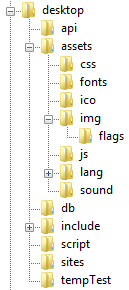
\includegraphics[width=0.25\textwidth]{images/folderStructure.png}
        \caption{The Code Folder Structure}
        \label{fig:folderStructure}
\end{figure}

\noindent{\textbf{web:} This is the main directory for the web interface.}\\
\\
\textbf{backend:} This is the main directory for the back end of the system.\\
\\
\textbf{api:} Is intended to contain API which are not JavaScript or PHP code.\\
\\
\textbf{assets:} Contains every asset in the system. Images, JavaScript, sound, fonts, CSS and language files.\\
\\
\textbf{assets - css:} Contains the CSS files for the system.\\
\\
\textbf{assets - fonts:} Contains special fonts for the system.\\
\\
\textbf{assets - ico:} Contains the icon files for the system.\\
\\
\textbf{assets - img:} Contains the static image resources for the system.\\
\\
\textbf{assets - img - flags:} Contains images of flags, used for changing language.\\
\\
\textbf{assets - js:} Contains all JavaScript in the system, files are named as they fit to PHP files, as far as this is possible.\\
\\
\textbf{assets - lang:} Contains all language files to the system. Each webpage and some JavaScripts, have their own language sub-folder .\\
\\
\textbf{db:} Contains the database files. All active database functions are stored in the file ``db.php''\\
\\
\textbf{include:} Contains any JavaScript or PHP code that is not developed by this project, but that is included in the system.\\
\\
\textbf{script:} Contains PHP scripts which do not display anything, but rather work to execute some functions.\\
\\
\textbf{sites:} Contains .html and .php files which correspond to a webpage on the web interface.\\
\\
\textbf{tempTest:} A folder for any need of generating files during development.

